\begin{frame}
  \frametitle{Características - Configuración de discos}
  \begin{itemize}
	  \item Configuración de discos IDE (\textit{Integrated Device Electronics}):
	  \begin{itemize}
	  	\item Master o Slave
	  	\item Primer y Segundo bus IDE
	  \end{itemize}
	  \item Denominación de los discos basada en los buses:
	  \begin{itemize}
	  	\item \textbf{/dev/hda}: configurado como Master en el 1º bus IDE
	  	\item \textbf{/dev/hdb}: configurado como Slave en el 1º bus IDE
	  	\item \textbf{/dev/hdc}: configurado como Master en el 2º bus IDE
	  	\item \textbf{/dev/hdd}: configurado como Slave en el 2º bus IDE
	  \end{itemize}
  \end{itemize}
\end{frame}

\begin{frame}
  \frametitle{Características - Configuración de discos (cont.)}
  \begin{itemize}
	  \item Configuración de discos SCSI: se basa en \textit{LUNS}
	  \item Denominación de los discos basada en la identificación de los buses:
	  \begin{itemize}
	  	\item \textbf{/dev/sda}
	  	\item \textbf{/dev/sdb}
	  	\item \textbf{/dev/sdc}
	  	\item \textbf{/dev/sdd}
	  	\item ...
	  \end{itemize}
	  \item La nomenclatura para los discos SATA es la misma
	  \item Particiones primarias:
	  \begin{itemize}
	  	\item Se numeran de la 1 a la 4 (solo estas se pueden marcar como activas $\rightarrow$ booteables)
	  \end{itemize}
	  \item Particiones extendidas:
	  \begin{itemize}
	  	\item Sus unidades o particiones lógicas se numeran a partir de la 5
	  \end{itemize}	  
  \end{itemize}
\end{frame}

\begin{frame}
  \frametitle{Características - Configuración de discos (cont.)}
  \begin{itemize}
	  \item Nueva nomenclatura utilizada:
	  \begin{itemize}
	  	\item Con la evolución de las distribuciones GNU/Linux, se comenzó a utilizar \textbf{``udev''} como gestor de dispositivos:
	  	\begin{itemize}
		  	\item Su función es controlar dinámicamente los archivos del /dev en base al hardware detectado
		  	\item Motiva su uso, el no poder garantizar que tras distintos arranques del SO, los dispositivos se sigan llamando de la misma manera. (Suponga disco 1 y 2, que disco 1 se quita y contorladoras SCSI/SATA mixtas)
		  	\item En /dev tendremos las entradas de los dispositivos conectados
		  	\item Desaparece el concepto de Major y Minor Number
		  	\item Se basa en eventos y permite que nuevos dispositivos sean agregados posteriormente al arranque
	  	\end{itemize}
	  \end{itemize}
  \end{itemize}
\end{frame}

\begin{frame}[fragile]
  \frametitle{Características - Configuración de discos (cont.)}
  \begin{itemize}
	  \item A futuro, todos los dispositivos llamados hdX serán denominados sdX $\leftarrow$ Introducido en Debian/Squeeze
	  \item Por estas y otras razones se adoptan 4 mecanismos nuevos para nomenclar los discos\footnote{\url{http://wiki.debian.org/Part-UUID}}:
	  \begin{itemize}
	  	\item Nombres persistentes por UUID (\tiny{Universal Unique Identifier}):
	  	\begin{lstlisting}
$ ls –l /dev/disk/by-uuid/
2d781b26-0285-421a-b9d0-d4a0d3b55680 -> ../../sda1
31f8eb0d-612b-4805-835e-0e6d8b8c5591 -> ../../sda7
		\end{lstlisting}
		\item Utilizando labels
		\begin{lstlisting}
$ ls -l /dev/disk/by-label
data -> ../../sdb2
data2 -> ../../sda2
		\end{lstlisting}
	  \end{itemize}
  \end{itemize}
\end{frame}

\begin{frame}
  \frametitle{Soporte de instalación}
  \begin{itemize}
	  \item Existen diversos modos de instalar GNU/Linux:
	  \begin{itemize}
	  	\item Debemos tener en cuenta la arquitectura de hardware
	  	\begin{itemize}
		  	\item amd64: Arquitectura de 64 bits
		  	\item arm ó armel: Advanced Risc Machine
		  	\item i386: Arquitectura de 32 bits
		  	\item ia64: intelItanium o Intel Architecture-64
		  	\item Otras
	  	\end{itemize}
	  	\item Podemos instalarlo desde un CD descargao de la web
	  	\item Podemos instalarlo desde un USB: Unetbootin
	  	\begin{itemize}
	  		\item Permite crear instaladores o LiveCD utilizando USBs
	  	\end{itemize}
	  \end{itemize}
  \end{itemize}
\end{frame}

\begin{frame}
  \frametitle{Herramientas para particionar}
  \begin{itemize}
	  \item El particionado de un disco se lo puede realizar mediante:
	  \begin{itemize}
	  	\item Software destructivo: \textit{fdisk}
	  	\item Software no destructivo: \textit{fips}, \textit{gparted}
		\begin{figure}
		    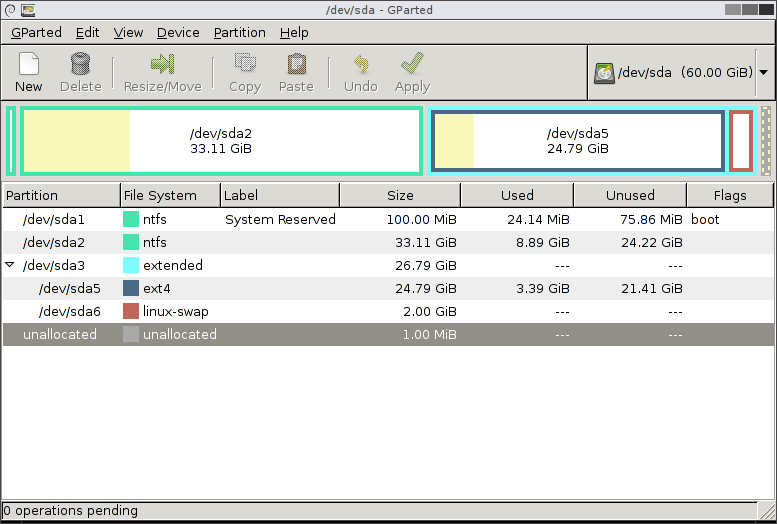
\includegraphics[scale=0.3]{images/gparted.png}
		\end{figure}
	  \end{itemize}
  \end{itemize}
\end{frame}

\begin{frame}
  \frametitle{Características}
  \begin{itemize}
	  \item No existe el concepto de \emph{extensión} en el nombre de un archivo
	  \item Los subdirectorios no se separan con el carácter `\textbackslash'
	  \item Es case sensitive
	  \item Entre un comando y sus parámetros debemos dejar obligatoriamente un espacio en blanco
	  \item Separación de entorno gráfico y texto
  \end{itemize}
\end{frame}

\begin{frame}
  \frametitle{Editor de textos \textbf{\emph{vim}}}
  \begin{itemize}
	  \item Presente en cualquier distribución de GNU/Linux
	  \item Posee 3 modos de ejecución:
	  \begin{itemize}
	  	\item Modo Insert
	  	\item Modo Visual
	  	\item Modo de Órdenes o Normal
	  \end{itemize}
	  \item Se le puede enviar una serie de comandos útiles
	  \begin{itemize}
	  	\item \textbf{w}: escribir cambios
	  	\item \textbf{q} ó \textbf{q!}: salir del editor
	  	\item \textbf{Ins} ó \textbf{i}: ingresar al modo edición
	  	\item \textbf{dd}: cortar
	  	\item \textbf{y}: copiar al portapapeles
	  	\item \textbf{p}: pegar desde el portapapeles
	  	\item \textbf{/}frase: busca ``frase'' dentro del archivo
	  \end{itemize}
  \end{itemize}
\end{frame}

\begin{frame}[fragile]
  \frametitle{Usuarios}
  \begin{itemize}
	  \item Todo usuario debe poseer credenciales para acceder al sistema
	  \begin{itemize}
	  	\item root: es el administrador del sistema (superusuario)
	  	\item otros: usuarios estándar del sistema (/etc/sudoers)
	  \end{itemize}
	  \item Archivos de configuración:
	  \begin{itemize}
	  	\item \textbf{/etc/passwd}
		\begin{lstlisting}
$ cat /etc/passwd
ndelrio:x:2375:500:Nico del Rio,,,,Usuarios:/home/admins/ndelrio:/bin/bash
		\end{lstlisting}	  	
	  	\item \textbf{/etc/group}
		\begin{lstlisting}
$ cat /etc/group		
infraestructura:x:500:
		\end{lstlisting}	  	
	  	\item \textbf{/etc/shadow}
		\begin{lstlisting}
$ cat /etc/shadow
ndelrio:$1$HamkgCYM$TtgfLJLplItxutaiqh/u9/:13273:0:99999:7:::
		\end{lstlisting}
	  \end{itemize}
  \end{itemize}
\end{frame}

\begin{frame}
  \frametitle{Usuarios (cont.)}
  \begin{itemize}
	  \item Comando para el manejo de usuarios:
	  \begin{itemize}
	  	\item \textbf{useradd} $<$nombreUsuario$>$:
	  	\begin{itemize}
	  		\item Agrega el usuario
	  		\item Modifica los archivos /etc/passwd
	  		\item Alternativa $\rightarrow$ \textbf{adduser}
	  	\end{itemize}
	  	\item \textbf{passwd} $<$nombreUsuario$>$:
	  	\begin{itemize}
	  		\item Asigna o cambia la contraseña del usuario
	  		\item Modifica el archivo /etc/shadow
	  	\end{itemize}
	  	\item \textbf{usermod} $<$nombreUsuario$>$:
	  	\begin{itemize}
	  		\item \textbf{-g}: modifica grupo de login (Modifica /etc/passwd)
	  		\item \textbf{-G}: modifica grupos adicionales (Modifica /etc/group)
	  		\item \textbf{-d}: modifica el directorio \emph{home} (Modifica /etc/passwd)
	  	\end{itemize}
	  	\item \textbf{userdel} $<$nombreUsuario$>$: elimina el usuario
	  	\item \textbf{groupdel} $<$nombreGrupo$>$: elimina el grupo
	  \end{itemize}
  \end{itemize}
\end{frame}

\begin{frame}[fragile]
  \frametitle{Permisos}
  \begin{itemize}
	  	\item Se aplican a directorios y archivos
	  	\item Existen 3 tipos de permisos y se basan en una notación octal:
	  	\begin{table}
		      \centering
		      \resizebox{10pc}{!}{
			  \begin{tabular}{| c | c | c |}
			      \hline
			      \bf Permiso & \bf Valor & \bf Octal \\
			      \hline
			      Lectura & R & 4 \\
			      \hline
			      Escritura & W & 2 \\
			      \hline
			      Ejecución & X & 1 \\
			      \hline
			  \end{tabular}
		      }
		\end{table}
		\item Se aplican sobre los usuarios:
		\begin{itemize}
			\item Usuario: permisos del dueño $\rightarrow$ \textbf{U}
			\item Usuario: permisos del grupo $\rightarrow$ \textbf{G}
			\item Usuario: permisos de otros usuario $\rightarrow$ \textbf{O}
		\end{itemize}
		\item Se utiliza el comando \textbf{chmod}:
		\begin{lstlisting}
$ chmod 755 /tmp/script
		\end{lstlisting}
  \end{itemize}
\end{frame}

\begin{frame}
  \frametitle{Entorno}
  \begin{itemize}
	  \item Algunos comandos útiles:
	  \begin{itemize}
	  	\item \textbf{ls}

	  	\item \textbf{cd}

	  	\item \textbf{mkdir}

	  	\item \textbf{rmdir}

	  	\item \textbf{rm}

	  	\item \textbf{mv}

	  	\item \textbf{cp}

	  	\item \textbf{man}
	  	
	  	\item \textbf{info}
	  \end{itemize}
  \end{itemize}
\end{frame}

\begin{frame}
  \frametitle{Bootloader}
  \begin{itemize}
  	\item El bootloader o cargador de arranque es un programa que permite cargar el Sistema Operativo. Puede llegar a cargar un entorno previo a la carga del sistema

  	\item Generalmente se utilizan los cargadores multietapas, en los que carios programas pequeños se van invocando hasta lograr la carga del SO

  	\item En cierto sentido, el código del \textit{BIOS} forma parte del bootloader, pero el concepto está más orientado al código que reside en el \textit{Master Boot Record} (512b)

  	\item El MBR está formado por el \textit{MBC} (446b) y la \textit{Tabla de Particiones} (64b)

  	\item Sólo el MBC del Primary Master Disk es tenido en cuenta

  	\item El MBR existe en todos los discos, ya que contiene la tabla de particiones
  \end{itemize}
\end{frame}

\begin{frame}
  \frametitle{Proceso de arranque \textbf{System V}}
  \begin{enumerate}
	\item Se empieza a ejecutar el código de la BIOS
	\item La BIOS ejecute el POST
	\item La BIOS lee el sector de arranque (MBR)
	\item Se carga el gestor de arranque (MBC)
	\item Se carga el kernel
	\item Se monta el sistema de archivos raíz (\textit{initrd}) y se inicializan componentes esenciales (e.j.: scheduling)
	\item Se ejecuta el proceso \textit{init}
	\item Lee el /etc/inittab
	\item Ejecuta los scripts apuntados por el \textit{runlevel 1}
	\item El final del runlevel 1 le indica que vaya al runlevel por defecto
	\item Ejecuta los scripts apuntados por el runlevel por defecto
	\item El sistema está listo para usarse
  \end{enumerate}
\end{frame}

\begin{frame}
  \frametitle{Proceso de arranque (cont.)}
  \begin{enumerate}
	\item su función es cargar todos los subproecos necesarios para el correcto funcionamiento del SO
	\item Posee el PID 1 y se encuentra en /sbin/init
	\item Se lo configura a través del archivo /etc/inittab en SysV
	\item No tiene padre y es el padre de todos los procesos (probar \textit{pstree})
	\item Es el encargado de montar los filesystems y de hacer disponible los demás dispositivos
  \end{enumerate}
\end{frame}

\begin{frame}[fragile]
  \frametitle{Runlevels}
  \begin{itemize}
	  	\item Es el modo en que arranca Linux (3 en \emph{Redhat}, 2 en \emph{Debian})
	  	\item El proceso de arranque lo dividimos en niveles. Cada un es responsable de leantar o bajar una serie de servicios
	  	\item Se encuentran definidos en /etc/inittab
	  	\textcolor{orange}{id:nivelesEjecución:acción:proceso}
		\begin{itemize}
			\item \textbf{Id}: identifica la entrada en inittab (1 a 4 carácteres)
			\item \textbf{NivelesEjecución}: el/los niveles de ejecución en los que se realiza la acción
			\item \textbf{Acción}: describe la acción a realizar
			\begin{itemize}
				\item \textbf{wait}: inicia cuando entra al runlevel e init espera a que termine
				\item \textbf{initdefault}
				\item \textbf{ctrlaltdel}: se ejecutará cuando init reciba la señal \emph{SIGINT}
				\item \textbf{off}, \textbf{respawn}, \textbf{once}, \textbf{boot}, \textbf{bootwait}, \textbf{powerwait}, etc.
			\end{itemize}
			\item \textbf{Proceso}: el proceso exacto que será ejecutado
		\end{itemize}
		\begin{lstlisting}
l1:1:wait:/etc/rc.d/rc 1
ca::ctrlaltdel:/sbin/shutdown -t3 -r
		\end{lstlisting}
  \end{itemize}
\end{frame}

\begin{frame}
  \frametitle{Proceso de arranque \textbf{Upstart}}
  \begin{itemize}
	  	\item Upstart es el reemplazo de SystemV (generalmente incluido en \emph{Ubuntu}, \emph{Fedora}, \emph{openSUSE}, etc.)
	  	\item Permite la ejecución de trabajos en forma asincrónica como principal diferencia con sysVinit que es estrictamente sincrónico
	  	\item Estos trabajos se denominan \textbf{jobs}
		\item El principal objetivo de un job es definir servicios o tareas a ser ejecutadas por init
		\item Son scripts de texto plano que definene las acciones/tareas (unidad de trabajo) a ejecutar ante determinados eventos
	  	\item Cada job es definido en el /etc/init
	  	\item Suelen ser de dos tipos:
	  	\begin{itemize}
	  		\item \textbf{Task}: ejecución finita (\textit{task}) $\rightarrow$ not respawning $\rightarrow$ exit 0 o uso de \textit{stop}
	  		\item \textbf{Service}: ejecución indeterminada $\rightarrow$ respawning
	  	\end{itemize}	  	
  \end{itemize}
\end{frame}

\begin{frame}
  \frametitle{Proceso de arranque \textbf{Upstart} (cont.)}
  \begin{itemize}
	  	\item Los jobs son ejecutados ante eventos (arranque del equipo, inserción de un dispositivo USB, etc.):
	  	\begin{itemize}
	  		\item Es posible crear eventos pero existen algunos de manera estándar\footnote{\url{http://people.canonical.com/~jhunt/upstart/upstart-states.png}}
	  		\item Definido por \textbf{start on} y \textbf{stop on}
	  	\end{itemize}  
  		\item Es compatible con SystemV $\rightarrow$ /etc/init/rc-sysinit.conf, runlevels, scripts en /etc/init.d
	  	\item Cada job posee un objetivo (\textit{goal}) y un estado (\textit{state})
	  	\begin{itemize}
	  		\item En base a ellos se ejecuta un proceso especifico
	  		\item Al inicio, init emite el evento \textit{startup}
	  	\end{itemize}
  \end{itemize}
\end{frame}

\begin{frame}
  	\frametitle{Proceso de arranque \textbf{Upstart} (cont.)}
  	\begin{itemize}
		\item Un job puede tener uno o varios procesos ejecutables como parte de su ciclo de vida y siempre debe existir el proceso principal
	  	\item Las tareas de un job se definen mediante \textit{exec} o \textit{script ... end script}
	  	\item A través de \textit{initctl} podemos administrar los jobs del demonio de Upstart:
	  	\begin{itemize}
	  		\item start $<$job$>$: cambia el objetivo a start del job especificado
	  		\item stop $<$job$>$: cambia el objetivo a stop del job especificado
	  		\item emit $<$event$>$: event es emitido causando que otros jobs cambien a objetivo start o stop
	  	\end{itemize}
  	\end{itemize}
\end{frame}